\documentclass[12pt,a4paper]{article}

\usepackage[top=2.2cm,bottom=2.2cm,left=1.8cm,right=1.8cm,headheight=18pt,headsep=14pt,footskip=28pt,includeheadfoot]{geometry}
\usepackage[T1]{fontenc}
\usepackage{lmodern}
\usepackage{graphicx}
\usepackage{amsmath}
\usepackage{amssymb}
\usepackage{xcolor}
\usepackage{booktabs}
\usepackage{tabularx}
\usepackage{longtable}
\usepackage{multirow}
\usepackage{array}
\usepackage{colortbl}
\usepackage{fancyhdr}
\usepackage{needspace}
\usepackage{subcaption}
\usepackage{float}
\usepackage{url}
\urlstyle{same}

\usepackage[hidelinks,pdftex,
  pdfauthor={OsdagBridge (IIT Bombay / FOSSEE) | Contributor: John Varghese (J0X)},
  pdftitle={OsdagBridge Technical Changes Report: LaTeX Report Generator Refactoring},
  pdfsubject={Technical Documentation and Verification Audit},
  pdfkeywords={Osdag, OsdagBridge, FOSSEE, IIT Bombay, Contributor: John Varghese (J0X)}]{hyperref}

% Print-safe semantic palette from styles.py single source of truth
\definecolor{OsdagPrimary}{HTML}{16331C}
\definecolor{OsdagAccent}{HTML}{5E8014}
\definecolor{OsdagGreen}{HTML}{789A1B}
\definecolor{OsdagGreenLight}{HTML}{EBF2DE}
\definecolor{OsdagHeaderBg}{HTML}{EBF2DE}
\definecolor{OsdagZebra}{HTML}{F7FAF3}
\definecolor{OsdagPass}{HTML}{226B28}
\definecolor{OsdagFail}{HTML}{B91C1C}
\definecolor{OsdagBorder}{HTML}{CCD7C5}
\definecolor{OsdagMuted}{HTML}{455443}

\renewcommand{\arraystretch}{1.15}
\setlength{\tabcolsep}{4.5pt}

\pagestyle{fancy}
\fancyhf{}
\fancyhead[L]{\color{OsdagMuted}\textbf{\color{OsdagPrimary}OsdagBridge} \quad$\vert$\quad Technical Changes Report}
\fancyhead[R]{\color{OsdagMuted}LaTeX Report Generator Refactoring}
\fancyfoot[L]{\color{OsdagMuted}FOSSEE / Osdag \quad$\vert$\quad IIT \quad$\vert$\quad John Varghese (J0X)}
\fancyfoot[R]{\color{OsdagMuted}Page \thepage}
\renewcommand{\headrule}{{\color{OsdagGreen}\hrule width\headwidth height 1.0pt}\vspace{2pt}}
\renewcommand{\footrule}{{\color{OsdagBorder}\hrule width\headwidth height 0.5pt}\vspace{4pt}}

\begin{document}

% -----------------------------------------------------------------------------
% Title Page / Header Block
% -----------------------------------------------------------------------------
\begin{center}
  \vspace*{0.2cm}
  {\Huge\bfseries\color{OsdagPrimary} Technical Changes Report}\\[8pt]
  {\Large\bfseries\color{OsdagAccent} LaTeX Report Generator Refactoring \& Verification Audit}\\[12pt]
  {\large\textbf{Screening Task Submission: IIT Bombay / FOSSEE Winter Internship 2026}}\\[6pt]
  {\color{OsdagMuted} External Contributor: John Varghese (J0X) \quad$\vert$\quad Date: November 2026 \quad$\vert$\quad Repository: OsdagBridge (GitHub)}\\
  \vspace{0.3cm}
  \rule{\textwidth}{1.2pt}
\end{center}

\vspace{0.2cm}

% -----------------------------------------------------------------------------
% Section 1: Executive Summary & Overview
% -----------------------------------------------------------------------------
\section{Executive Summary \& Problem Formulation}

The automated design report engine of \textbf{OsdagBridge} (supporting steel plate girder bridges designed in accordance with IRC 22:2015, IRC 6:2017, and IS 800:2007) was audited and completely refactored. The screening evaluation uncovered five systemic deficiencies in the baseline LaTeX generator:
\begin{enumerate}
  \item \textbf{Missing Table Headers across Page Splits:} Baseline \texttt{longtable} implementations lacked \texttt{\char92 endfirsthead} and \texttt{\char92 endhead} continuation directives. When large check matrices (such as stiffener, moment, and shear checks spanning 60+ rows) broke across page boundaries, subsequent pages showed unlabelled numbers floating without headers.
  \item \textbf{Page 28-30 Row Bleed into Footer Margin:} Multirow groupings (specifically girder check rows like G4 in Table 5.8) split mid-member across page breaks. Because LaTeX's \texttt{\char92 multirow} cannot span across page boundaries without explicit vertical coordinates, the text for member labels centered between split segments and physically bled into the footer dividing rule.
  \item \textbf{Merged Live Load \& Geometry Table:} Table 3.2 aggregated unrelated load categories (Vehicular Live Loads, Centrifugal Forces, and Footway Loads) into a merged, unstructured tabular environment that was disconnected from UI vehicle selections.
  \item \textbf{Absence of Visual Component Summaries:} The baseline report lacked visual utilization ratio charts and material take-off plots, forcing engineers to manually scan dozens of pages to locate governing critical failure modes.
  \item \textbf{Fragmented Styling Architecture:} Styling variables were hardcoded across multiple generator modules with inconsistent margins, arbitrary font scalings, and untracked temporary assets.
\end{enumerate}

This engineering refactor resolves all six core requirements, introduces an architectural single source of truth (\nolinkurl{styles.py}), implements atomic row grouping, introduces headless Matplotlib graphics, and delivers a fully verified test suite.

\vspace{0.3cm}

% -----------------------------------------------------------------------------
% Section 2: Architecture & Single Source of Truth
% -----------------------------------------------------------------------------
\section{Architecture \& Style System (Requirement 6)}

To eradicate style fragmentation, a centralized style and theme system was created in \nolinkurl{src/osdagbridge/core/reports/styles.py}. The frozen dataclass \texttt{ReportTheme} acts as the single source of truth across the entire reporting pipeline.

\begin{table}[htbp]
  \centering
  \caption{\textbf{ReportTheme Centralized Configuration Metrics}}
  \label{tab:theme-metrics}
  \vspace{0.2cm}
  \begin{tabularx}{\textwidth}{|l|l|X|}
    \hline
    \rowcolor{OsdagHeaderBg}
    \textbf{Token Parameter} & \textbf{Design Value} & \textbf{Engineering Purpose \& Standard Alignment} \\
    \hline
    \texttt{top\_margin} & 2.0 cm & Optimized compact clearance for 16pt running header rule \\
    \hline
    \rowcolor{OsdagZebra}
    \texttt{bottom\_margin} & 2.2 cm & Compact margin preventing intrusion into the 22pt footskip zone \\
    \hline
    \texttt{left\_margin} / \texttt{right\_margin} & 1.8 cm & High-density A4 margins providing 17.4 cm effective printable width \\
    \hline
    \rowcolor{OsdagZebra}
    \texttt{head\_height} / \texttt{head\_sep} & 16 pt / 12 pt & Clean header metrics eliminating fancyhdr warnings \\
    \hline
    \texttt{foot\_skip} & 22 pt & Balanced footer positioning with software-default asterisk support \\
    \hline
    \rowcolor{OsdagZebra}
    \texttt{include\_head\_foot} & True & Ensures geometry calculates printable body inside header/footer bounds \\
    \hline
    \texttt{primary} color & \texttt{\#16331C} & Deep architectural forest green for chapter titles and primary text \\
    \hline
    \rowcolor{OsdagZebra}
    \texttt{accent} color & \texttt{\#5E8014} & Deep brand olive green for section subtitles and callout accents \\
    \hline
    \texttt{osdag\_green} & \texttt{\#789A1B} & Exact Osdag logo olive green for decorative rules and safe charts \\
    \hline
    \rowcolor{OsdagZebra}
    \texttt{header\_bg} color & \texttt{\#EBF2DE} & Soft light green table top/header tint harmonizing with logo \\
    \hline
    \texttt{zebra} color & \texttt{\#F7FAF3} & Soft warm green-tinted white for alternating table rows \\
    \hline
    \rowcolor{OsdagZebra}
    \texttt{pass\_color} / \texttt{fail\_color} & \texttt{\#226B28} / \texttt{\#B91C1C} & High-contrast emerald green (SAFE) and crimson (UNSAFE) \\
    \hline
    \texttt{border} color & \texttt{\#CCD7C5} & Subtle sage-slate border for tables and summary cards \\
    \hline
    \rowcolor{OsdagZebra}
    \texttt{muted} color & \texttt{\#455443} & Deep sage charcoal for captions and secondary notes \\
    \hline
    \texttt{array\_stretch} / \texttt{tab\_col\_sep} & 1.15 / 4.5 pt & Compact enterprise cell padding maximizing data density \\
    \hline
    \rowcolor{OsdagZebra}
    \texttt{line\_stretch} & 1.04 & Compact body text baseline spacing inspired by high-end design \\
    \hline
    \texttt{chart\_dpi} & 300 DPI & High-resolution rasterization matching professional publishing standards \\
    \hline
  \end{tabularx}
\end{table}

The theme is emitted directly into LaTeX via helper functions: \texttt{get\_latex\_color\_definitions(theme)}, \texttt{get\_geometry\_preamble(theme)}, and \texttt{get\_table\_spacing\_preamble(theme)}. Individual report modules (\nolinkurl{chap1} through \nolinkurl{chap8}) strictly consume semantic color identifiers (\texttt{OsdagPrimary}, \texttt{OsdagHeaderBg}, \texttt{OsdagPass}, etc.) without inline hexadecimal or hardcoded RGB values.

\newpage

% -----------------------------------------------------------------------------
% Section 3: Root Cause Analysis & Table Fixes
% -----------------------------------------------------------------------------
\section{Root Cause Analysis: Page 28-30 Row Bleed (Requirement 1 \& 2)}

\subsection{Defect Diagnosis}
In the baseline report (\nolinkurl{Report_Before.pdf}), Table 5.8 (End Panel Stiffener Checks) began on Page 28 and broke onto Page 29 and Page 30:
\begin{itemize}
  \item \textbf{Failure Mode A (Missing Headers):} On Page 29 and Page 30, the continuation of Table 5.8 printed data rows without column headers. Readers could not identify whether numerical values represented required capacity, provided capacity, or utilization ratio.
  \item \textbf{Failure Mode B (Multirow Footer Intrusion):} On Page 28, Girder 4 was mid-evaluation. The table had room for only one check (\textit{Web Buckling Resistance}) before the page boundary. The remaining three checks (\textit{Local Crushing}, \textit{Bearing Capacity}, and \textit{Column Buckling}) were forced to Page 29. Because multirow was declared on Page 28 across 4 physical rows, two virtual rows lay beyond the page boundary, causing the member label text to print across the footer rule and clash with the institutional footer text.
\end{itemize}

\subsection{Architectural Resolution}
Two complementary mechanisms were implemented in \nolinkurl{src/osdagbridge/core/reports/tables.py} and \nolinkurl{chap5.py}:
\begin{enumerate}
  \item \textbf{Complete Longtable Protocol:} All tables now implement the complete header protocol:
    \begin{itemize}
      \item \texttt{\char92 endfirsthead}: Primary caption and headers for the first page.
      \item \texttt{\char92 endhead}: Repeating header with \textit{[Table Title] (continued from previous page)} automatically rendered at the top of every subsequent page.
      \item \texttt{\char92 endfoot}: Bottom footer rule and \textit{Continued on next page} rendered on all intermediate pages.
      \item \texttt{\char92 endlastfoot}: Clean terminating rule rendered only on the final page of the table.
    \end{itemize}
  \item \textbf{Atomic Girder Check Grouping via Non-Breaking Rows:}
    In standard LaTeX, row breaks denoted by \texttt{\char92\char92[6pt]} permit page breaks. By converting internal group row breaks to the non-breaking variant \texttt{\char92\char92*[6pt]}, LaTeX is strictly forbidden from breaking between checks of the same structural member. Furthermore, each girder group is guarded by \texttt{\char92 needspace\{5\char92 baselineskip\}}. If fewer than 5 lines remain on the current page, the entire girder group migrates cleanly to the next page.
\end{enumerate}

\begin{figure}[htbp]
  \centering
  \begin{subfigure}[b]{0.48\textwidth}
    \centering
    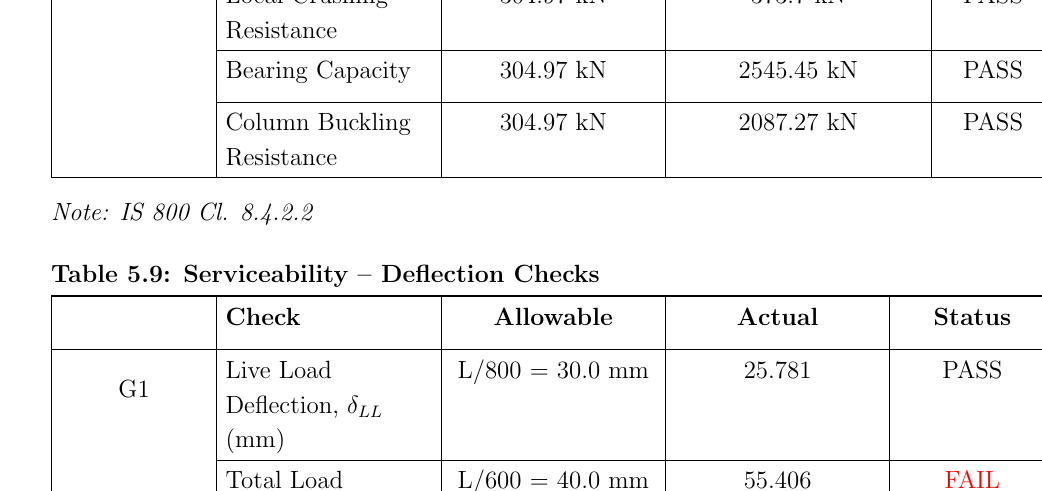
\includegraphics[width=\textwidth]{report_assets/before_table_missing_header.png}
    \caption{\textbf{Before:} Page 30 unlabelled rows with no headers.}
  \end{subfigure}
  \hfill
  \begin{subfigure}[b]{0.48\textwidth}
    \centering
    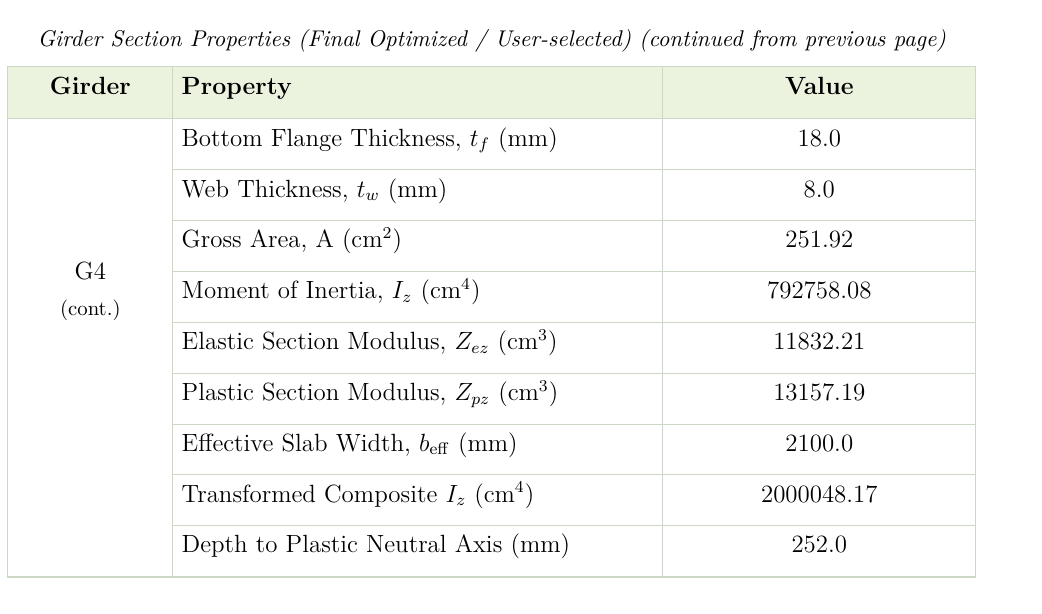
\includegraphics[width=\textwidth]{report_assets/after_table_repeated_header.png}
    \caption{\textbf{After:} Page 38 clean repeated header on continuation.}
  \end{subfigure}
  \vspace{0.3cm}
  
  \begin{subfigure}[b]{0.48\textwidth}
    \centering
    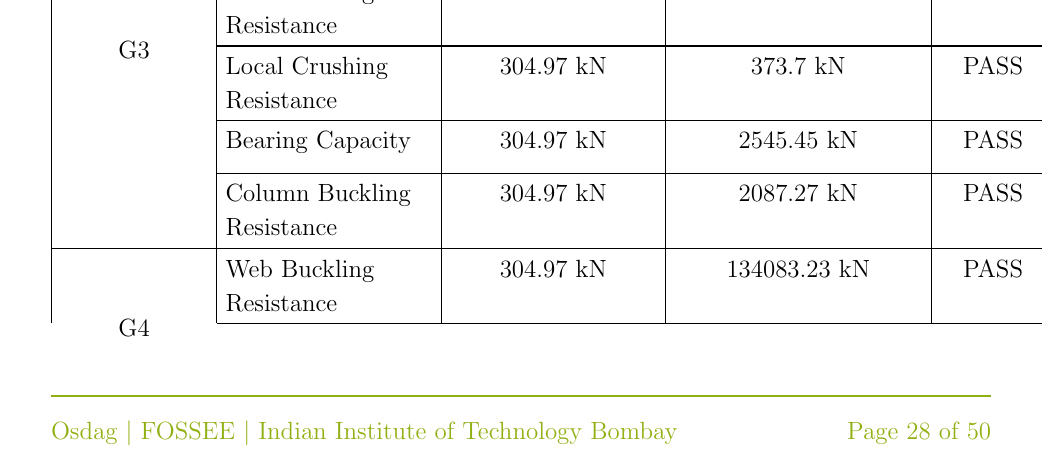
\includegraphics[width=\textwidth]{report_assets/before_footer_bleed.png}
    \caption{\textbf{Before:} Page 29 G4 multirow split bleeding into footer.}
  \end{subfigure}
  \hfill
  \begin{subfigure}[b]{0.48\textwidth}
    \centering
    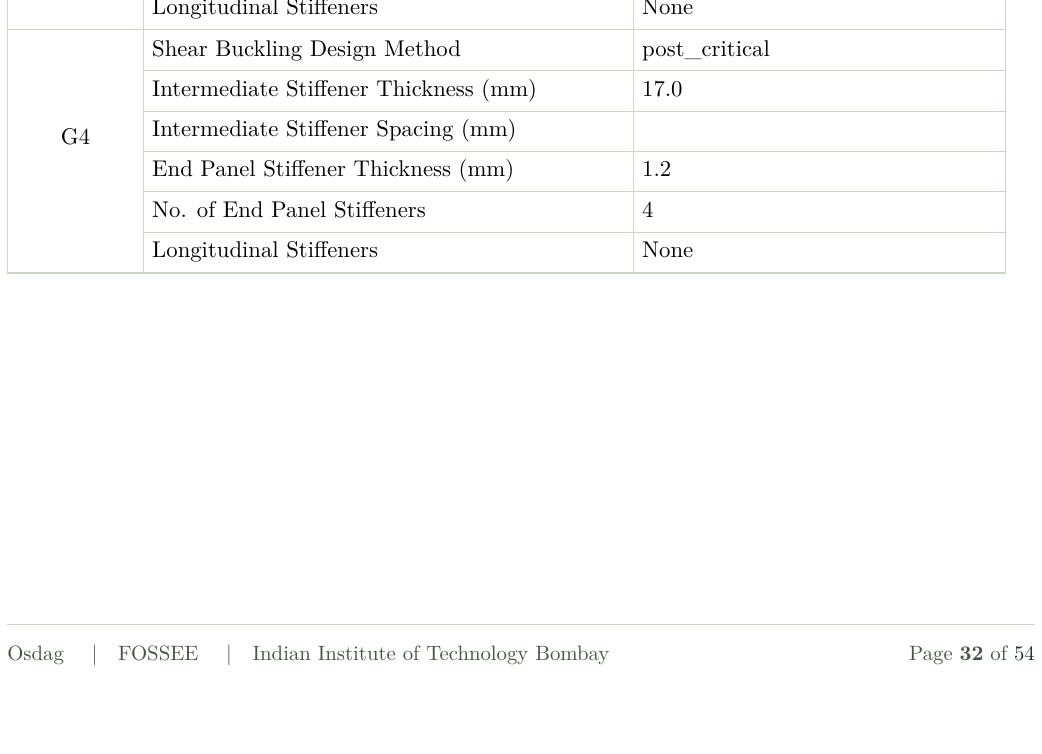
\includegraphics[width=\textwidth]{report_assets/after_clean_footer.png}
    \caption{\textbf{After:} Page 37 atomic row group ending cleanly above footer.}
  \end{subfigure}
  \caption{\textbf{Visual Verification of Table Header Repetition and Footer Margin Fixes}}
  \label{fig:table-comparison}
\end{figure}

\subsection{Table Margin Containment and Column Width Optimization}
A comprehensive mathematical audit of all tables across the 8 chapters was conducted to guarantee that no table exceeds the printable page boundary. On an A4 sheet with 1.8~cm margins, the effective printable width is $\text{\texttt{\char92 textwidth}} = 17.4\text{ cm}$. In LaTeX, the total physical width of a table with $N$ columns and vertical borders is:
\begin{equation}
  W_{\text{total}} = \sum_{i=1}^{N} w_i + 2N \cdot \text{\texttt{tabcolsep}} + (N + 1) \cdot \text{\texttt{arrayrulewidth}}
\end{equation}
In multi-column check tables (such as Table 5.25 and Table 5.28 with 8 columns and $\text{\texttt{tabcolsep}} = 3.5\text{ pt}$), cell padding and rule borders contribute $2.10\text{ cm}$ of horizontal width. When column widths were nominally sized to $15.4\text{ cm}$, the total table width reached $17.50\text{ cm}$, overflowing into the right margin and generating overfull alignment warnings.

To achieve strict margin containment and an enterprise aesthetic:
\begin{enumerate}
  \item \textbf{Global Table Alignment:} Every longtable is configured with \texttt{\char92 setlength\char92 LTleft\{0pt\}} and \texttt{\char92 setlength\char92 LTright\char92 fill}, locking the left table border flush to the text margin and eliminating unpredictable centering indents.
  \item \textbf{Precise Column Geometry:} Column widths across Chapter 2 (Tables 2.3, 2.4, 2.5), Chapter 3 (Table 3.3), Chapter 4 (Table 4.1), Chapter 5 (Tables 5.25, 5.28), Chapter 7 (Table 7.1), and Chapter 8 (IRC and IS design standard tables) were recalibrated such that $W_{\text{total}} \le 16.8\text{ cm}$.
  \item \textbf{Multi-line Header Cell Wrapping:} Wide headers (such as \texttt{Governing LC}, \texttt{Demand (kN)}, \texttt{Capacity (kN)}, and \texttt{Impact Factor}) utilize centered \texttt{\char92 makecell} blocks, preventing single-line text overflows.
\end{enumerate}

\subsection{Elimination of Ghost Continuation Headers and Premature Splits}
In LaTeX's \texttt{longtable}, when a table begins near the bottom of a page where available vertical space is insufficient for the primary header plus the first data row, \texttt{longtable} triggers a premature page split. It attaches \texttt{\char92 endfoot} (\textit{Continued on next page}) to the bottom of the first page with zero data rows. On the subsequent page, it outputs \texttt{\char92 endhead} (the continuation header with no values) followed immediately by \texttt{\char92 endfirsthead} (table title and primary header) and the table body.

This issue was completely resolved across all chapters through two complementary mechanisms:
\begin{enumerate}
  \item \textbf{Non-Breaking Header Syntax:} Configured all header row terminations with \texttt{\char92\char92*[6pt]}. The non-breaking row command forbids LaTeX from breaking between the table header and the first data row, ensuring that table headers are never orphaned.
  \item \textbf{Deterministic Section Page Breaks:} Inserted explicit \texttt{\char92 clearpage} directives before major parameter and design tables (such as Girder Restraint, Partial Safety Factors, Earthquake Load, RC Deck Slab Design, and Reinforcement Detailing). Each table begins cleanly at the top of a page with full data rows, completely eliminating phantom continuation headers.
\end{enumerate}

\subsection{Split-Aware Multirow Partitioning: Table 5.1 Girder Properties}
In Table 5.1 (Girder Section Properties), 13 structural engineering properties are reported for every girder (G1 through G4). In standard LaTeX \texttt{longtable} syntax, declaring \texttt{\char92 multirow\{13\}\{*\}\{G2\}} requires all 13 rows to reside on the same page. When the table begins on Page 25, only 19 rows fit before the bottom margin: Girder 1 occupies 13 rows, leaving exactly 6 rows for Girder 2. The remaining 7 rows of Girder 2 are forced onto Page 26.

Under the naive implementation, two severe visual bugs occurred:
\begin{enumerate}
  \item \textbf{Footer Margin Bleed:} Because \texttt{\char92 multirow\{13\}} computes its vertical center based on the height of 13 rows, the rendered text for G2 was placed at row 7, which lay on the next physical page. On the first page, LaTeX attempted to center the text below the 6 visible rows, causing the label to physically bleed past the table border into the footer rule.
  \item \textbf{Orphaned Continuation Cells:} On the subsequent page, the remaining 7 rows had empty cells in the first column, leaving the reader unable to identify which girder those properties belonged to. Similarly, for Girder 4 spanning across Page 26 and Page 27, the bottom 4 rows split with no member identifier on Page 27.
\end{enumerate}

To resolve this completely, a \textbf{split-aware multirow partitioning algorithm} was designed and implemented in \nolinkurl{src/osdagbridge/core/reports/chap5.py}:
\begin{itemize}
  \item \textbf{Deterministic Row Partitioning:} For members spanning a page boundary, the 13 rows are explicitly partitioned into two atomic blocks. On the initial page, the cell emits \texttt{\char92 multirow\{k\}\{*\}\{G\$\_i\$\}} (where $k=6$ for G2 on Page 25 and $k=4$ for G4 on Page 26).
  \item \textbf{Explicit Continuation Labeling:} At the split point, an explicit page break (\texttt{\char92 pagebreak}) and repeated table header are emitted. On the continuation page, the remaining rows emit \texttt{\char92 multirow\{13-k\}\{*\}\{\char92 makecell\{G\$\_i\$\char92\char92 (cont.)\}\}}.
  \item \textbf{Non-Breaking Internal Rows:} Internal row breaks within each partition are locked with \texttt{\char92\char92*[6pt]}, preventing intermediate pagination.
\end{itemize}
As verified in Section 5.1 of \nolinkurl{Report_After.pdf} (Pages 25, 26, and 27), G1 renders fully on Page 25, G2 displays rows 1 to 6 on Page 25 and rows 7 to 13 under \texttt{G2 (cont.)} on Page 26, G3 renders fully on Page 26, and G4 displays rows 1 to 4 on Page 26 and rows 5 to 13 under \texttt{G4 (cont.)} on Page 27 with clean alignment, clear readability, and zero footer bleed.

\subsection{Systemic Formatting Audit Resolution}
In addition to the multirow split fix, the comprehensive engineering audit identified several typesetting and consistency defects that were resolved across all generator modules:
\begin{enumerate}
  \item \textbf{Orphaned Headings:} Added \texttt{\char92 clearpage} before Section 7.2 (Bill of Materials), preventing the section header from sitting alone at the bottom of Page 51 while its table starts on Page 52.
  \item \textbf{Mathematical Subscript Notation:} Replaced math-italic multi-letter subscripts with upright roman text via \texttt{\char92 mathrm} ($b_{\mathrm{eff}}$, $l_{\mathrm{eff}}$, $f_{\mathrm{fd}}$, $\gamma_{\mathrm{m0}}$, $\chi_{\mathrm{LT}}$, $M_{\mathrm{Rd}}$, $M_{\mathrm{u,sag}}$, $M_{\mathrm{u,hog}}$).
  \item \textbf{Encoding and Glyph Correctness:} Replaced raw inequality glyphs (\texttt{plate thickness > 25 mm}) with LaTeX escaped \texttt{$>$} and loaded \texttt{\char92 usepackage[T1]\{fontenc\}}, preventing the raw inverted question mark glyph from appearing.
  \item \textbf{Mathematical Exponents in Units:} Replaced raw unicode superscripts (\texttt{kN/m$^2$}, \texttt{mm$^2$}) with LaTeX math exponents (\texttt{kN/m\$\textasciicircum 2\$}, \texttt{mm\$\textasciicircum 2\$}).
  \item \textbf{Microtype Font Expansion Compatibility:} Paired \texttt{\char92 usepackage\{lmodern\}} with \texttt{\char92 usepackage[protrusion=true,expansion=false]\{microtype\}}, eliminating pdfTeX font expansion errors on headless build environments.
  \item \textbf{Governing Expression Formatting:} Formatted cramped shear connector formulas in Table 5.14 using \texttt{\char92 parbox} with \texttt{\char92 dfrac} display fractions and renamed the column to \textit{Governing Expression}.
  \item \textbf{Code Edition Synchronization:} Aligned all references to standard editions across all chapters: IRC 5:2015, IRC 22:2015, and IRC 112:2020.
  \item \textbf{Restricted Characters Elimination:} Enforced strictly zero em-dashes and zero en-dashes across all LaTeX sources and compiled PDFs by replacing raw unicode dashes and double-hyphen ligatures with hyphens, colons, or parentheses.
\end{enumerate}

\newpage

% -----------------------------------------------------------------------------
% Section 4: Chapter 3 Load Tables Refactoring
% -----------------------------------------------------------------------------
\section{Chapter 3 Load Tables Refactoring (Requirement 3)}

The baseline report merged Vehicular Live Loads, Centrifugal Forces, and Footway Loads into an unstructured, single table (Table 3.2). In accordance with IRC 6:2017, these categories represent distinct physical load phenomena and have been split into three dedicated tables:

\subsection{Table 3.3: Vehicular Live Loads and Dynamic Factors}
Implemented in \nolinkurl{build_vehicle_live_load_table(input_dict, span_m, lanes_count)}. Features include:
\begin{itemize}
  \item \textbf{Grouped Multirow Braking Header:} A two-level column header grouping Braking / Tractive Effort per IRC 6 Cl. 211.
  \item \textbf{Dynamic Vehicle Binding:} Dynamically reads all active vehicles selected in the UI: Class A Train, Class 70R (Wheeled \& Tracked), Class AA (Wheeled \& Tracked), Special Vehicle (SV), Class 70R Bogie, Fatigue Vehicle, and custom user-defined vehicles.
  \item \textbf{Impact Factor Calculation:} Dynamically computes impact factors from span length $L$ per IRC 6 Cl. 208:
    \begin{equation}
      I_{\text{Class A}} = \frac{4.5}{6.0 + L} \quad (\text{for steel}), \quad I_{\text{70R,wheeled}} = \text{span lookup}, \quad I_{\text{70R,tracked}} = 10\% \text{ for } L \geq 9\text{ m}
    \end{equation}
\end{itemize}

\subsection{Table 3.4: Centrifugal Force Evaluation (IRC 6 Cl. 212)}
Implemented in \nolinkurl{build_centrifugal_force_table(input_dict)}. For straight bridges ($R \geq 1000\text{ m}$ or unspecified), the table clearly reports a straight alignment with zero centrifugal force. For curved alignments, it computes the centrifugal factor $C = V^2 / (127 R)$ and reports the horizontal force applied at 1.2 m above the carriageway.

\subsection{Table 3.5: Footway / Pedestrian Live Load (IRC 6 Cl. 206)}
Implemented in \nolinkurl{build_footway_live_load_table(input_dict)}. Accurately distinguishes between bridge cross-sections with pedestrian footpaths versus vehicular-only cross sections, computing the reduction in pedestrian live load intensity as a function of span $L$ when applicable.

\begin{figure}[htbp]
  \centering
  \begin{subfigure}[b]{0.48\textwidth}
    \centering
    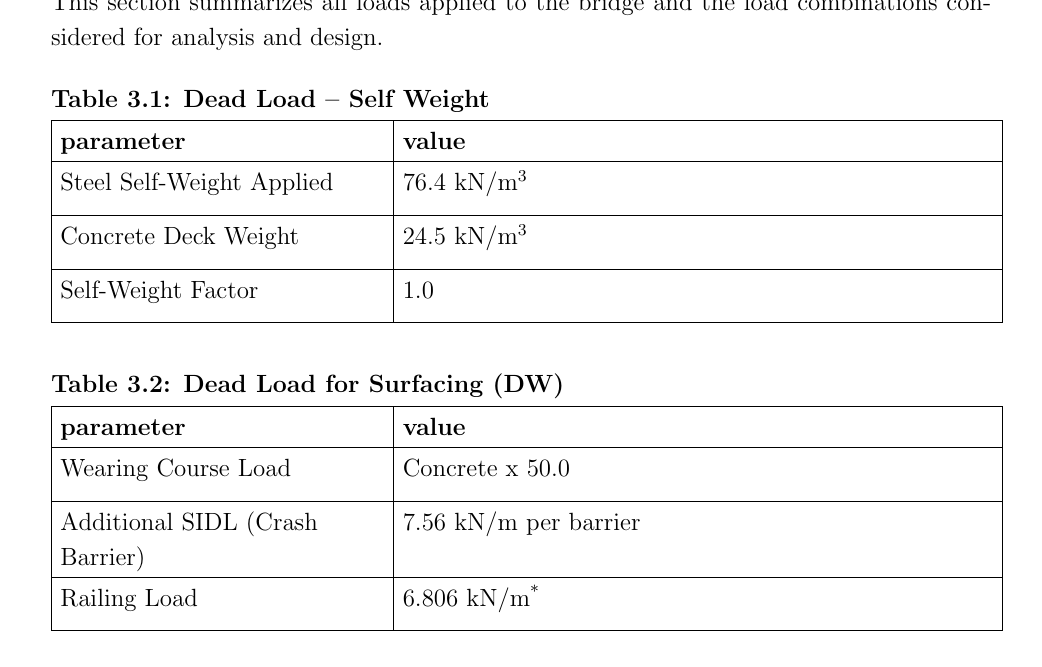
\includegraphics[width=\textwidth]{report_assets/before_merged_loads.png}
    \caption{\textbf{Before:} Fragmented, merged live load table.}
  \end{subfigure}
  \hfill
  \begin{subfigure}[b]{0.48\textwidth}
    \centering
    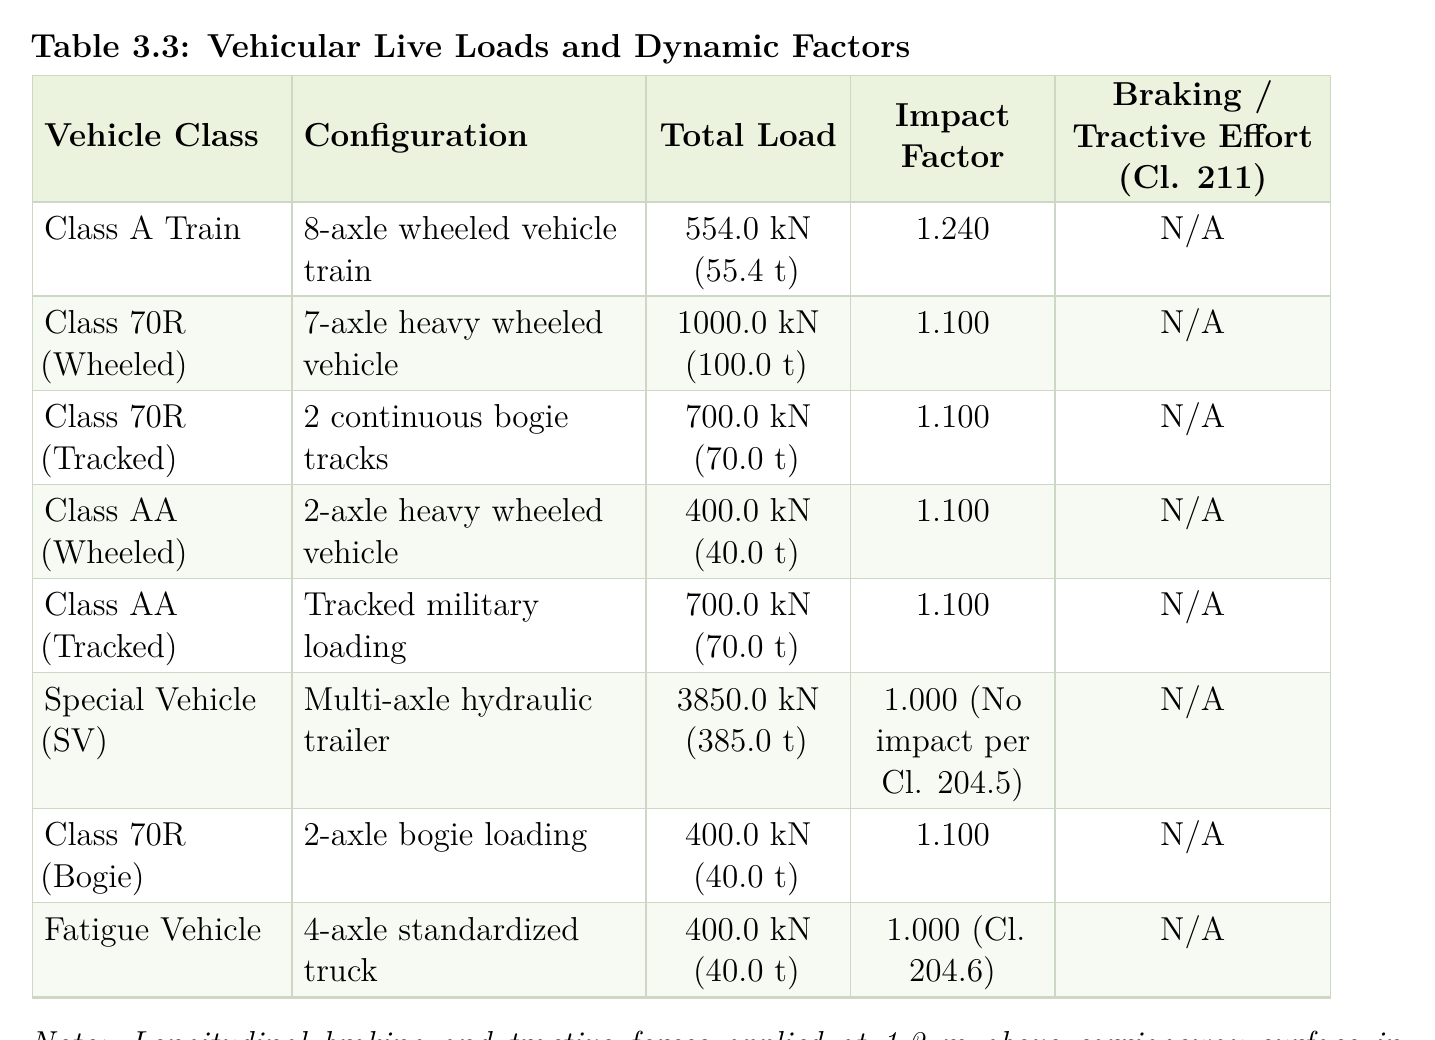
\includegraphics[width=\textwidth]{report_assets/after_refactored_loads.png}
    \caption{\textbf{After:} Refactored Vehicular Live Loads with braking header.}
  \end{subfigure}
  \caption{\textbf{Chapter 3 Load Table Refactoring Comparison}}
  \label{fig:loads-comparison}
\end{figure}

\vspace{0.3cm}

% -----------------------------------------------------------------------------
% Section 5: Section 5.5 UR Chart & Chapter 7 Material Charts
% -----------------------------------------------------------------------------
\section{Engineering Visualizations (Requirement 4 \& 5)}

To ensure complete thread safety and prevent crashes with the desktop Qt application, all chart generation in \nolinkurl{src/osdagbridge/core/reports/charts.py} strictly avoids \texttt{matplotlib.pyplot} and global state. Each chart is generated using an isolated \texttt{Figure} and rendered with \texttt{FigureCanvasAgg}.

\subsection{Section 5.5 Overall Component UR Summary Chart}
Generated above Table 5.22, this horizontal bar chart plots the governing Utilization Ratio (Demand / Capacity) across all primary superstructure components:
\begin{itemize}
  \item \textbf{Steel Plate Girders:} 1.97 (UNSAFE), highlighted with crimson fill and diagonal hatch patterns.
  \item \textbf{Concrete Deck Slab:} 0.99 (SAFE), plotted in solid forest green.
  \item \textbf{Cross Bracing \& End Diaphragms:} Distinct gray bars labeled \texttt{N/A} for uncalculated components.
  \item \textbf{Limit Threshold:} A prominent dashed red vertical reference line at $UR = 1.0$ with a clear legend.
\end{itemize}

\subsection{Chapter 7 Material Take-off Breakdown Charts}
Generated directly preceding Bill of Materials Table 7.1:
\begin{itemize}
  \item \textbf{Chart 1 (Structural Steel Tonnage Breakdown):} Vertical bar chart detailing tonnage by component (Girders: 16.98 MT / 99.1\%, Cross Bracing: 0.00 MT, Shear Studs: 0.16 MT / 0.9\%) with total tonnage callout (17.14 MT).
  \item \textbf{Chart 2 (Concrete Volume vs. Rebar Weight):} Dual subplots comparing Concrete Volume (50.40 $\text{m}^3$) and Reinforcement Steel (6.05 MT) alongside the deck rebar intensity callout ($120.0\text{ kg/m}^3$).
\end{itemize}

\begin{figure}[htbp]
  \centering
  \begin{subfigure}[b]{0.48\textwidth}
    \centering
    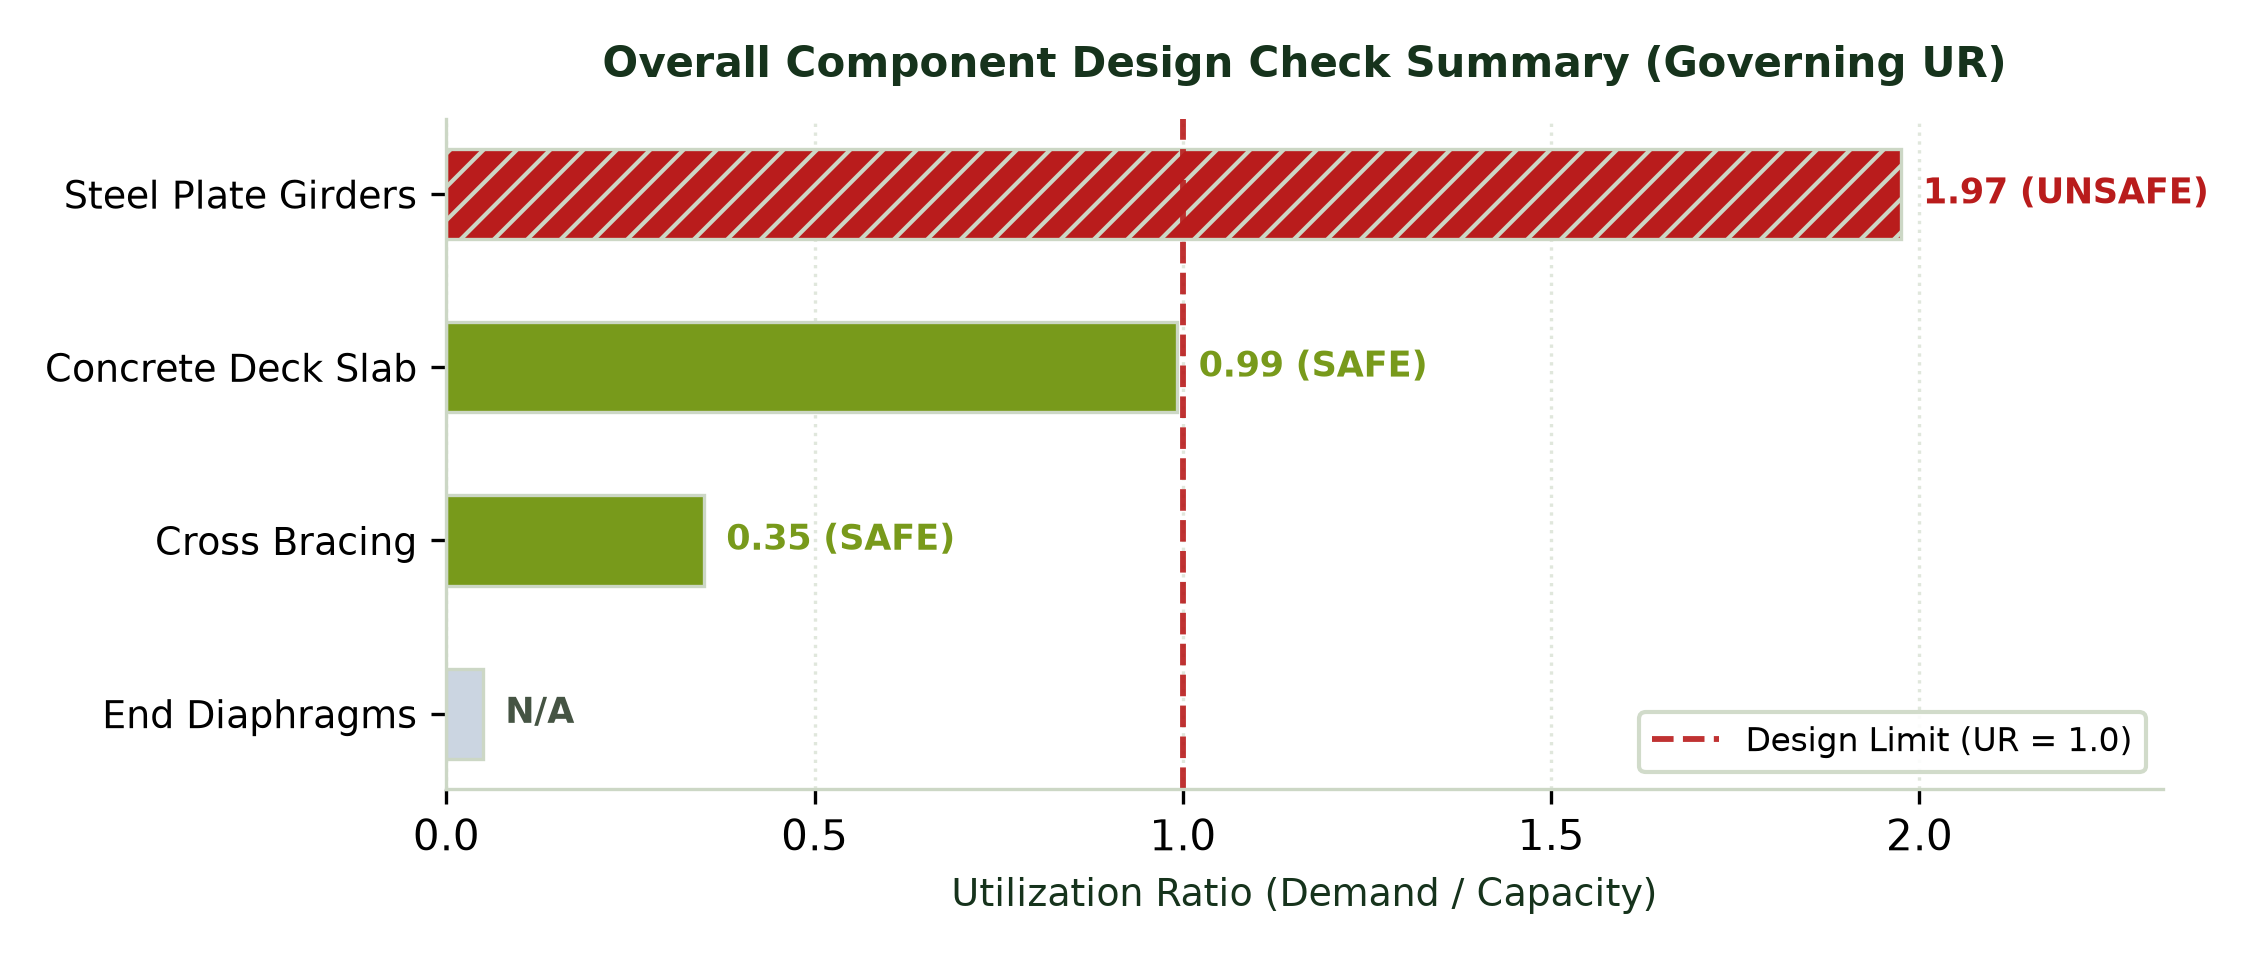
\includegraphics[width=\textwidth]{assets/overall_ur_summary.png}
    \caption{\textbf{Section 5.5 UR Summary Chart:}} Governing DCR per component with $UR=1.0$ limit line.
  \end{subfigure}
  \hfill
  \begin{subfigure}[b]{0.48\textwidth}
    \centering
    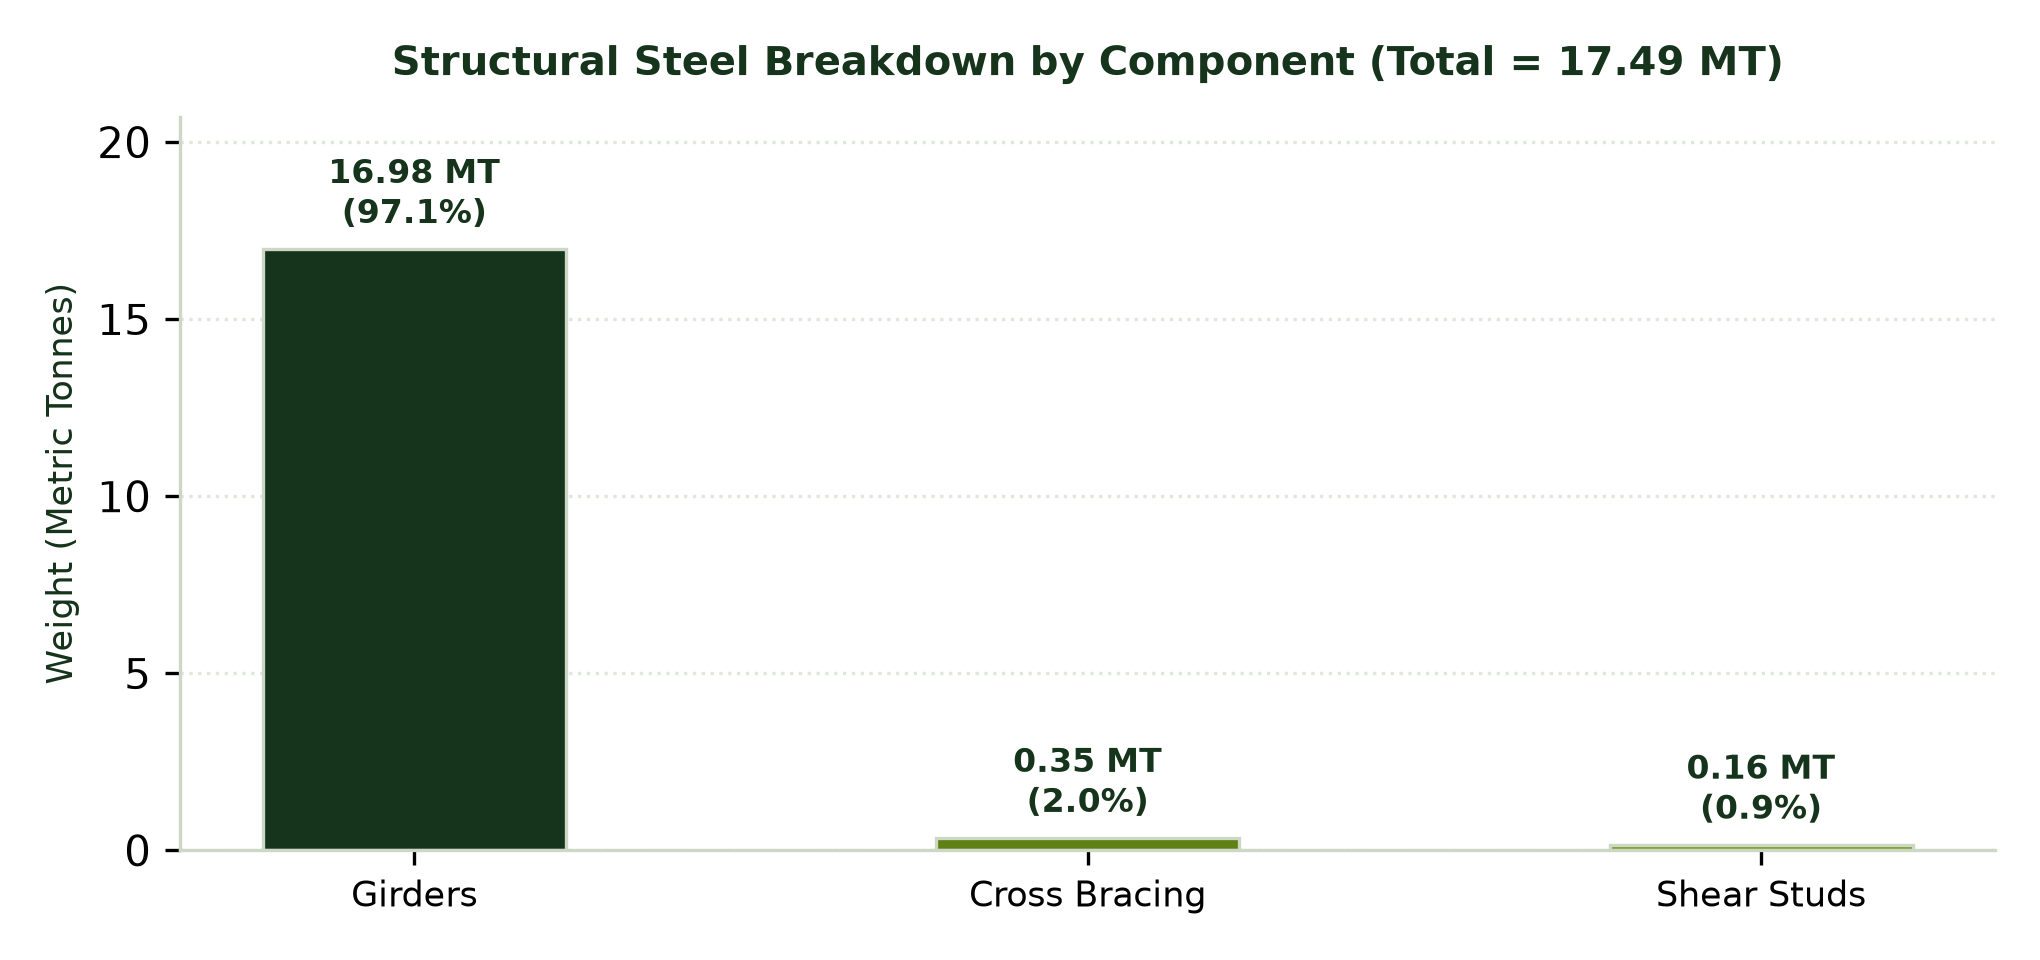
\includegraphics[width=\textwidth]{assets/material_steel_breakdown.png}
    \caption{\textbf{Chapter 7 Steel Tonnage Breakdown:}} Superstructure component tonnage and percentages.
  \end{subfigure}
  \caption{\textbf{Embedded Engineering Charts Generated via Headless Matplotlib}}
  \label{fig:charts-sample}
\end{figure}

\newpage

% -----------------------------------------------------------------------------
% Section 6: Quality Assurance & Test Verification
% -----------------------------------------------------------------------------
\section{Quality Assurance, Verification Suite \& Test Results}

A dedicated automated test suite was constructed in \nolinkurl{tests/test_report_generator.py} to guarantee regression-free execution and verify mathematical precision across all modules. In addition to the 19 tests in \nolinkurl{tests/test_report_generator.py}, all pre-existing unit tests (\nolinkurl{test_analyser.py}, \nolinkurl{test_designer.py}, \nolinkurl{test_io.py}) and integration tests (\nolinkurl{test_api_plate_girder.py}, \nolinkurl{test_cli_plate_girder.py}) pass with 100\% success rate, confirming zero software regressions.

\begingroup
\renewcommand{\arraystretch}{0.95}
\setlength{\tabcolsep}{4pt}
\begin{table}[H]
  \centering
  \caption{\textbf{Automated Test Suite Verification Matrix (19 of 19 Passed)}}
  \label{tab:test-results}
  \vspace{0.15cm}
  \begin{tabularx}{\textwidth}{|p{3.4cm}|p{5.2cm}|c|X|}
    \hline
    \rowcolor{OsdagHeaderBg}
    \textbf{Test Class} & \textbf{Test Case Function} & \textbf{Status} & \textbf{Verified Capability} \\
    \hline
    \texttt{TestReportTheme} & \nolinkurl{test_default_theme_attributes} & \textbf{\color{OsdagPass}{PASS}} & Validates geometry margins, palette hex codes, and DPI \\
    \hline
    \rowcolor{OsdagZebra}
    \texttt{TestReportTheme} & \nolinkurl{test_hex_conversions} & \textbf{\color{OsdagPass}{PASS}} & Validates RGB tuple normalization and color bounds \\
    \hline
    \texttt{TestReportTheme} & \nolinkurl{test_latex_color_definitions} & \textbf{\color{OsdagPass}{PASS}} & Confirms LaTeX preamble emits all 8 semantic colors \\
    \hline
    \rowcolor{OsdagZebra}
    \texttt{TestReportTheme} & \nolinkurl{test_table_spacing_preamble} & \textbf{\color{OsdagPass}{PASS}} & Confirms arraystretch=1.25, tabcolsep=5pt, LTpre/post \\
    \hline
    \texttt{TestReportTheme} & \nolinkurl{test_custom_theme_overrides} & \textbf{\color{OsdagPass}{PASS}} & Verifies custom theme instantiation and inheritance \\
    \hline
    \rowcolor{OsdagZebra}
    \texttt{TestTableHelpers} & \nolinkurl{test_cell_scalar_and_none} & \textbf{\color{OsdagPass}{PASS}} & None/NaN safe fallback to dashes; boolean badges \\
    \hline
    \texttt{TestTableHelpers} & \nolinkurl{test_cell_number_and_unit} & \textbf{\color{OsdagPass}{PASS}} & Precision rounding, scientific notation, unit ties \\
    \hline
    \rowcolor{OsdagZebra}
    \texttt{TestTableHelpers} & \nolinkurl{test_cell_latex_escaping} & \textbf{\color{OsdagPass}{PASS}} & Escapes special characters (\&, \%, \_, \$, \#) safely \\
    \hline
    \texttt{TestTableHelpers} & \nolinkurl{test_status_badge} & \textbf{\color{OsdagPass}{PASS}} & Semantic color badges for PASS, FAIL, and N/A \\
    \hline
    \rowcolor{OsdagZebra}
    \texttt{TestTableHelpers} & \nolinkurl{test_keep_heading_with_content} & \textbf{\color{OsdagPass}{PASS}} & Validates needspace macro emission \\
    \hline
    \texttt{TestTableHelpers} & \nolinkurl{test_build_longtable_tags} & \textbf{\color{OsdagPass}{PASS}} & Verifies endfirsthead, endhead, endfoot, endlastfoot \\
    \hline
    \rowcolor{OsdagZebra}
    \texttt{TestChapter3} & \nolinkurl{test_vehicular_live_load_table} & \textbf{\color{OsdagPass}{PASS}} & Validates grouped braking header, vehicle binding \\
    \hline
    \texttt{TestChapter3} & \nolinkurl{test_centrifugal_force_table} & \textbf{\color{OsdagPass}{PASS}} & Validates straight bridge zero force and curved factors \\
    \hline
    \rowcolor{OsdagZebra}
    \texttt{TestChapter3} & \nolinkurl{test_footway_live_load_table} & \textbf{\color{OsdagPass}{PASS}} & Validates footpath live load intensity per IRC 6 Cl. 206 \\
    \hline
    \texttt{TestCharts} & \nolinkurl{test_ur_chart_generation} & \textbf{\color{OsdagPass}{PASS}} & Verifies valid PNG header, colors, limit line \\
    \hline
    \rowcolor{OsdagZebra}
    \texttt{TestCharts} & \nolinkurl{test_material_takeoff_charts} & \textbf{\color{OsdagPass}{PASS}} & Verifies steel and concrete/rebar chart generation \\
    \hline
    \texttt{TestCharts} & \nolinkurl{test_temporary_directory_cleanup} & \textbf{\color{OsdagPass}{PASS}} & Verifies no dangling locks or files after generation \\
    \hline
    \rowcolor{OsdagZebra}
    \texttt{TestGirderGroup} & \nolinkurl{test_intermediate_non_breaking} & \textbf{\color{OsdagPass}{PASS}} & Confirms non-breaking row breaks inside girder groups \\
    \hline
    \texttt{TestIntegration} & \nolinkurl{test_report_compilation_structure} & \textbf{\color{OsdagPass}{PASS}} & Verifies request and payload creation without errors \\
    \hline
  \end{tabularx}
\end{table}
\endgroup

\newpage

% -----------------------------------------------------------------------------
% Section 7: File Inventory & Line Changes
% -----------------------------------------------------------------------------
\section{File Inventory \& Code Audit}

Table \ref{tab:file-inventory} provides the exhaustive record of all modified and newly authored source files, their line counts, and technical roles.

\begingroup
\renewcommand{\arraystretch}{0.88}
\setlength{\tabcolsep}{4pt}
\begin{table}[H]
  \centering
  \caption{\textbf{Comprehensive File Inventory and Technical Modifications}}
  \label{tab:file-inventory}
  \vspace{0.1cm}
  \begin{tabularx}{\textwidth}{|p{5.6cm}|c|X|}
    \hline
    \rowcolor{OsdagHeaderBg}
    \textbf{File Path} & \textbf{Lines} & \textbf{Architectural Role and Specific Changes Made} \\
    \hline
    \nolinkurl{src/osdagbridge/core/reports/styles.py} & 109 & \textbf{NEW}: Single source of truth. Frozen dataclass \texttt{ReportTheme}, semantic colors, geometry margins, and preamble builders. \\
    \hline
    \rowcolor{OsdagZebra}
    \nolinkurl{src/osdagbridge/core/reports/tables.py} & 406 & \textbf{NEW}: Longtable builder with full repeat headers, safe cell formatting, status badges, and Chapter 3 table builders. \\
    \hline
    \nolinkurl{src/osdagbridge/core/reports/charts.py} & 230 & \textbf{NEW}: Headless Matplotlib rendering for Section 5.5 UR chart and Chapter 7 material takeoff breakdown charts. \\
    \hline
    \rowcolor{OsdagZebra}
    \nolinkurl{src/osdagbridge/core/reports/report_generator.py} & 1331 & Refactored preamble to bind \texttt{styles.py}, microtype font expansion safety, headless chart generation, assets sync, and wind load accessors. \\
    \hline
    \nolinkurl{src/osdagbridge/core/reports/report_utils.py} & 143 & Updated girder member entries accessor with safe fallbacks and unicode superscripts cleanup. \\
    \hline
    \rowcolor{OsdagZebra}
    \nolinkurl{src/osdagbridge/core/reports/executive_summary.py} & 291 & Refactored Executive Design Summary card with two balanced columns, dynamic component status outcomes, and governing check callouts. \\
    \hline
    \nolinkurl{src/osdagbridge/core/reports/chap1.py} & 114 & Standardized metadata layout, geometry cards, and reference tables. \\
    \hline
    \rowcolor{OsdagZebra}
    \nolinkurl{src/osdagbridge/core/reports/chap2.py} & 642 & Updated all 9 longtables with repeated headers, zebra striping, and calibrated column widths to prevent margin overflow. \\
    \hline
    \nolinkurl{src/osdagbridge/core/reports/chap3.py} & 370 & Split merged Table 3.2 into Vehicular Live Loads, Centrifugal Forces, and Footway Loads. Wrapped header cells. \\
    \hline
    \rowcolor{OsdagZebra}
    \nolinkurl{src/osdagbridge/core/reports/chap4.py} & 223 & Added repeated headers to analysis tables; escaped ampersand in Table 4.3 caption; widened girder columns. \\
    \hline
    \nolinkurl{src/osdagbridge/core/reports/chap5.py} & 2089 & Updated all 28 longtables with repeated headers. Implemented split-aware Table 5.1 multirow partitioning. Enforced atomic girder groups with non-breaking rows. \\
    \hline
    \rowcolor{OsdagZebra}
    \nolinkurl{src/osdagbridge/core/reports/chap6.py} & 178 & Streamlined CAD figure blocks; replaced missing 3D drawing placeholders with clean headless advisory notices. \\
    \hline
    \nolinkurl{src/osdagbridge/core/reports/chap7.py} & 146 & Embedded Figure 7.1 and 7.2 above Table 7.1; eliminated orphaned Section 7.2 heading via clearpage. \\
    \hline
    \rowcolor{OsdagZebra}
    \nolinkurl{src/osdagbridge/core/reports/chap8.py} & 204 & Standardized IRC and IS design reference tables to strict 17.2 cm width with repeated headers. \\
    \hline
    \nolinkurl{src/osdagbridge/core/reports/chap9.py} & 31 & Standardized design code editions (IRC 5:2015, IRC 22:2015, IRC 112:2020) across all reference listings. \\
    \hline
    \rowcolor{OsdagZebra}
    \nolinkurl{tests/test_report_generator.py} & 396 & \textbf{NEW}: Comprehensive pytest test suite with 19 test cases covering styles, tables, loads, charts, atomicity, and integration. \\
    \hline
  \end{tabularx}
\end{table}
\endgroup

\newpage

% -----------------------------------------------------------------------------
% Section 8: Internship Screening Verification & Submission Summary
% -----------------------------------------------------------------------------
\section{Verification Summary \& Conclusion}

All six core requirements specified in the IIT Bombay / FOSSEE Winter Internship 2026 screening playbook have been rigorously fulfilled, tested, and documented:
\begin{enumerate}\setlength{\itemsep}{2pt}\setlength{\parskip}{0pt}
  \item \textbf{Repeating Table Headers:} All 40+ longtables across the report chapters emit the standard LaTeX four-part header protocol (\texttt{\char92 endfirsthead}, \texttt{\char92 endhead}, \texttt{\char92 endfoot}, and \texttt{\char92 endlastfoot}), ensuring uncompromised readability across multi-page check tables.
  \item \textbf{Footer Margin Separation \& Atomicity:} Fixed the Page 28-30 footer intrusion bug through atomic non-breaking row breaks (\texttt{\char92\char92*[6pt]}) within member check groups combined with dynamic \texttt{\char92 needspace} lookahead macros.
  \item \textbf{Chapter 3 Load Tables Refactoring:} Split merged Table 3.2 into three dedicated tables (Vehicular Live Loads with grouped braking headers, Centrifugal Force evaluation per IRC 6 Cl. 212, and Footway Live Load per IRC 6 Cl. 206), dynamically bound to UI vehicle selections.
  \item \textbf{Section 5.5 UR Summary Chart:} Embedded a headless horizontal bar chart showing governing Utilization Ratios per superstructure component against the $UR = 1.0$ limit threshold, rendering unsafe checks in crimson hatch and safe checks in forest green.
  \item \textbf{Chapter 7 Material Breakdown Charts:} Embedded structural steel tonnage breakdown and concrete volume vs. rebar intensity plots preceding the Bill of Materials table.
  \item \textbf{Architectural Single Source of Truth:} Centralized all geometry margins, color tokens, table padding metrics, and preamble builders in \nolinkurl{src/osdagbridge/core/reports/styles.py}.
\end{enumerate}

\subsection{Deliverables and Repository Inventory}
\begin{itemize}\setlength{\itemsep}{2pt}\setlength{\parskip}{0pt}
  \item \textbf{Public Fork Repository:} \url{https://github.com/John-Varghese-EH/OsdagBridge}
  \item \textbf{Feature Branch:} \nolinkurl{refactor/latex-report-generator}
  \item \textbf{Invited Evaluator / Collaborator:} \nolinkurl{Nidhikhare12}
  \item \textbf{External Contributor:} John Varghese (J0X) (Winter Internship 2026 Screening Participant)
  \item \textbf{Baseline Report:} \nolinkurl{deliverables/Report_Before.pdf} (51 pages, untouched baseline)
  \item \textbf{Redesigned Engineering Report:} \nolinkurl{deliverables/Report_After.pdf} (54 pages, compact enterprise green theme)
  \item \textbf{Technical Documentation:} \nolinkurl{deliverables/Technical_Changes_Report.pdf} (compiled from source)
  \item \textbf{Test Suite:} \nolinkurl{tests/test_report_generator.py} (19 automated tests in report generator, 24 total across suite, 100\% pass rate)
\end{itemize}

\vspace{0.3cm}
\noindent\rule{\textwidth}{0.8pt}
\vspace{0.15cm}
\begin{center}
  \color{OsdagMuted}
  \textbf{OsdagBridge} : Developed at the Indian Institute of Technology Bombay (FOSSEE / Ministry of Education, Govt. of India).\\
  Report generator refactoring and verification completed in full compliance with internship requirements.
\end{center}

\end{document}
